\section{Semana 2 - Market Opportunities, Costs, Addicional Design Generation and Analytic Hierarchy Process (AHP)}
\subsection{Market Opportunities}
\subsection{Costs}
\subsection{Addicional Design Generation}
\subsubsection{Introdução}
Na semana dois, foi necessário realizar o Analytic Hierarchy Process (AHP). Este consiste num método para avaliar designs comparativamente. Dado que foi decidido que este deveria avaliar quatro designs, consideramos outros dois adicionais para além dos detalhados na secção referente à semana anterior a esta.\par

\subsubsection{Lillium jet, ductos, e aviões elétricos}
Dada a convencionalidade do dois primeiros designs esboçados, de forma a procurar criar conceitos variados para o AHP, foi decidido investigar aeronaves menos convencionais, nomeadamente no ramo de mobilidade urbana e regional. Dever-se-á notar que, primeiramente, foi focada a procura de soluções puramente a combustão e baseado em aeronaves exprimentais e já em serviço, de forma a confirmar a viabilidade das nossas escolhas. Alargou-se, assim, neste ponto do trabalho, a procura, em particular, para eVTOL.\par
Vários designs existentes de veiculos eVTOL foram considerados e uma lista dos candidatos que pareceram mais viáveis e mais interessantes para o nosso projeto foi compilada:
\begin{itemize}
    \item Joby S4 - pelo mecanismo de tilt rotor
    \item NASA Greased Lightning - pelo mecanismo de tilt wing
    \item NASA LA-8 - pelo mecanismo de tilt wing e tandem wing
    \item HopFlyt Venturi - pelo design de channel wings e tandem wing
    \item Airbus A³ Vahana - pelo design tandem wing extremamente semelhante ao inicialmente considerado
    \item Bell Nexus 6HX - pelo design de ducted fans
    \item Lillium Jet - pelo design de tandem wing com micropropulsão de ducted jets 
\end{itemize}
Desta pesquisa resultou a escolha do Lillium Jet como referência, dado ser uma das aeronaves mais avançadas no seu desenvolvimento, e com características que melhor se alinhavam com os nossos objetivos, nomeadamente o seu pequeno tamanho juntamente com a redução de ruído e aumento de eficiência e segurança prometidos pelo seu design de jatos elétricos. 
O Lillium Jet apresenta uma configuração fixed wing com canard, puramente elétrica de propulsão distribuída com jatos em ductos embebidos que podem ser rodados para descolagem e aterragem vertical. Uma imagem representativa é apresentada em baixo.\par
\FloatBarrier
\begin{figure}[h]
    \begin{subfigure}[t]{0.47\textwidth}
        \centering
        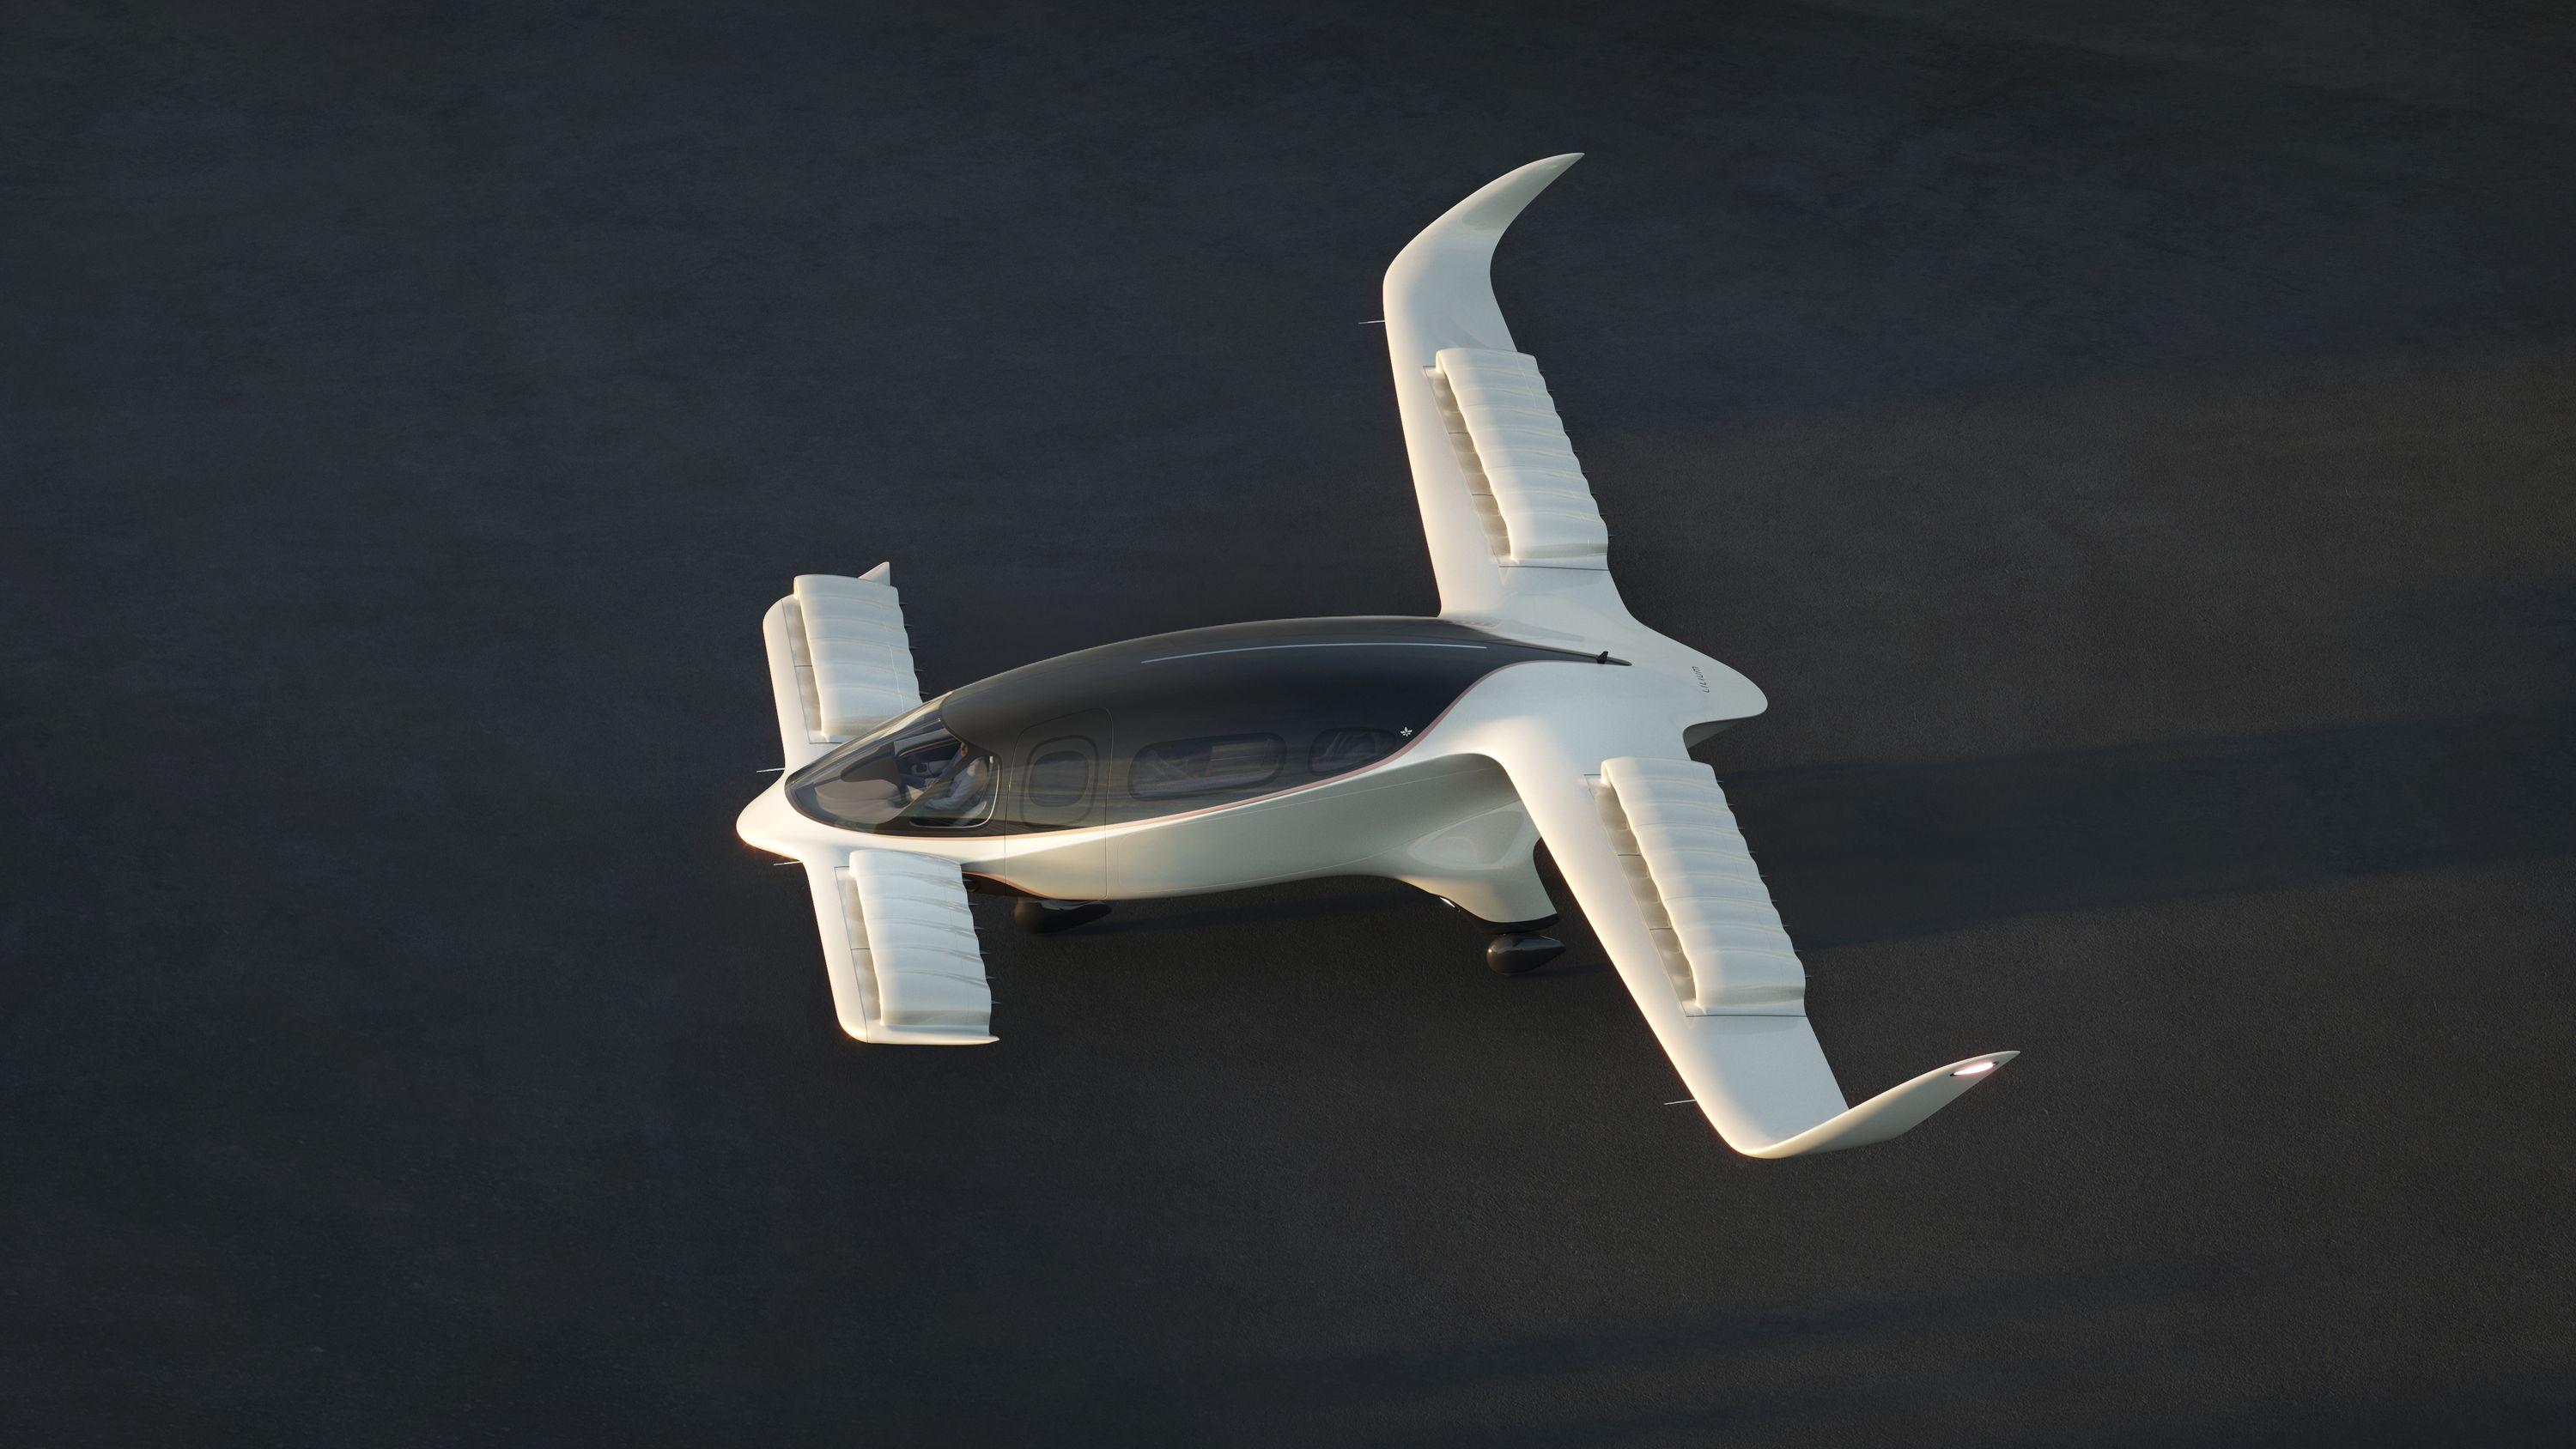
\includegraphics[width=\textwidth]{Imagens/Lilium-Jet-Top-Side_result1.jpg}
        \caption{Lillium Jet Source:\cite{noauthor_2022-ne}}
        \label{LilliumJet}
    \end{subfigure}
    \hfill
    \begin{subfigure}[t]{0.47\textwidth}
        \centering
        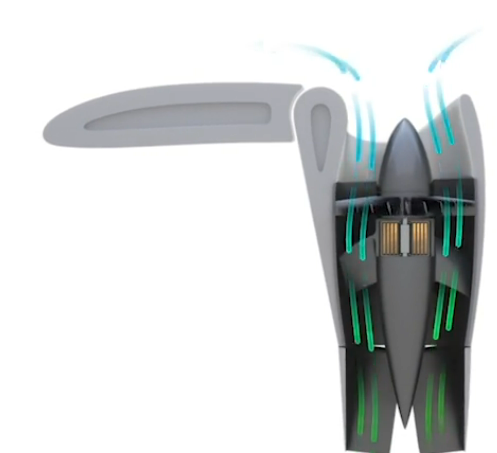
\includegraphics[width=\textwidth]{Imagens/tiltrotorlillium.PNG}
        \caption{Lillium Jet Source:\cite{noauthor_2022-ne}}
        \label{LilliumJettiltrotor}
    \end{subfigure}
    \caption{Lillium Jet e detalhe da propulsão}
\end{figure}
\FloatBarrier
O uso de jatos em ductos sobre a asa deve resultar numa maior eficiência em todo o perfil de voo bem como numa redução de ruído durante a operação. Tal se deve à diminuição das interações entre os rotores e o isolamento acústico inerente a cobrir os rotores, à diminuição dos números de Mach locais (equivalente a permitir que os rotores possam rodar mais rapidamente, melhorando a sua eficiência), ao uso de tubeiras convergentes para obter maior impuslo com um rotor menor, e ao facto de que ao estarem colocados no bordo de fuga acelerarem o o ar sobre a asa, criando lift adicional. Têm no entanto a desvantagem de adicionarem peso e complexidades estruturais à aeronave, além de serem mais difíceis de prever aerodinamicamente ao contrario de configurações convencionais. {\large{\textbf{citaç~eos para isto tudo, s'il vous plait}}}\par
Além da existência de ductos, este desgin também se distingue ao usar 36 pequenos motores elétricos distribuídos ao longo da asa e do canard.
Tendo em conta o apresentado, foi considerado que o fator mais distinto e importante era o sistema de propulsão, pelo que se baseou os novos designs nos primeiros, modificando-os para fazerem uso de tilt jets embebidos na asa, tal como o Lillium Jet. Em baixo encontram-se os novos designs apresentados na segunda semana.
\FloatBarrier
\begin{figure}[h]
    \centering
    \begin{subfigure}[b]{0.47\textwidth}
        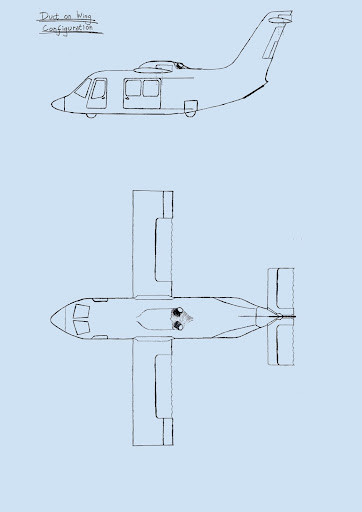
\includegraphics[width=\textwidth]{Imagens/segundodesign1.jpg}
        \caption{Segundo Design Sketch 1}
        \label{SecondDesingSketchini1}
    \end{subfigure}
    \hfill
    \begin{subfigure}[b]{0.47\textwidth}
        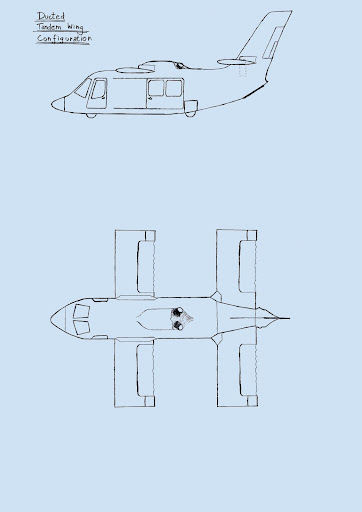
\includegraphics[width=\textwidth]{Imagens/segundodesign2.jpg}
        \caption{Segundo Design Sketch 2}
        \label{SecondDesingSketchini2}
    \end{subfigure}
    \caption{Conceitos com propulsão distribuída  - Semana 2}
\end{figure}
\FloatBarrier
Dever-se-á notar, então, que, no topo das asas, encontram-se motores elétricos de dimensões menores aos apresentados na semana um. Estes, tal como no Lillium Jet, encontram-se no bordo de fuga e deverão ter como exequivel a mudança de orientação através dum mecanismo semelhante àquele presente no Lillium Jet, em particular expressado na figura \ref{LilliumJettiltrotor}.\par
\subsection{Analytic Hierarchy Process (AHP)}
\textbf{HOnestamente, não me apetece escrever isto pq eu nem percebi bem o pq de decidirmos que certos parametros são melhores que os outros, so ya||| pois eu tb nem quero ter de me lembrar que sequer fizemos esta parvoice da AHP de adivinhar o que era bom e mau para depois concluirmos "adivinhamos errado"}